\section{Two-Dimensional Systems}
\noindent\rule[\linienAbstand]{\linewidth}{\linienDickeDick}
We now consider the systmes for arbitrary $n \in \mathbb(N)$, i.e.
\begin{equation}
  \begin{split}
    \dot{x}_1 &= f_1(x_1, x_2,...,x_n)\\
    \dot{x}_2 &= f_2(x_1, x_2,...,x_n)\\
     &\;\;...\\
    \dot{x}_n &= f_n(x_1, x_2,...,x_n)
  \end{split}
\end{equation}
resp. in vector notation
\begin{equation}
  \dot{\mathbf{x}} = \mathbf{f}(\mathbf{x}) \;\;\; (\mathbf{x}\in\mathbb(R)^n)
\end{equation}



\textbf{Definitions}\\
A point $x^* \in \mathbb{R}^n$ is a \emph{fixed point} of the dynamical system $\dot{\mathbf{x}} =  \mathbf{f}(\mathbf{x})$, if
\begin{equation}
  \mathbf{f}(\mathbf{x^*}) = \mathbf{0}
\end{equation}
If $\mathbf{x^*}$ is a \emph{fixed point} of the dynamical system $\dot{\mathbf{x}} =  \mathbf{f}(\mathbf{x})$, then
\begin{equation}
   \mathbf{x}(t) =  \mathbf{x}^*
\end{equation}
is a constant solution.\\

A fixed point $x^* \in \mathbb{R}^n$ of the dynamical system $\dot{\mathbf{x}} =  \mathbf{f}(\mathbf{x})$, is
\begin{itemize}
  \item \emph{stable}, if the solution starting close to $x^*$ stays close to $x^*$ for all $t \geq 0$.
  \item \emph{asymptotically stable}, if the solution starting close to $x^*$ converge to $x^*$ for $t \rightarrow \infty$.
  \item \emph{unstable}, if the solution starts close to $x^*$ and diverging from $x^*$ for $t \rightarrow \infty$.
\end{itemize}

\subsection{Linear Systems}
\noindent\rule[\linienAbstand]{\linewidth}{\linienDicke}

Overview over the various types of fixed points and the corresponding geometry of the system near the fixed point:
\begin{figure}[H]
  \centering
  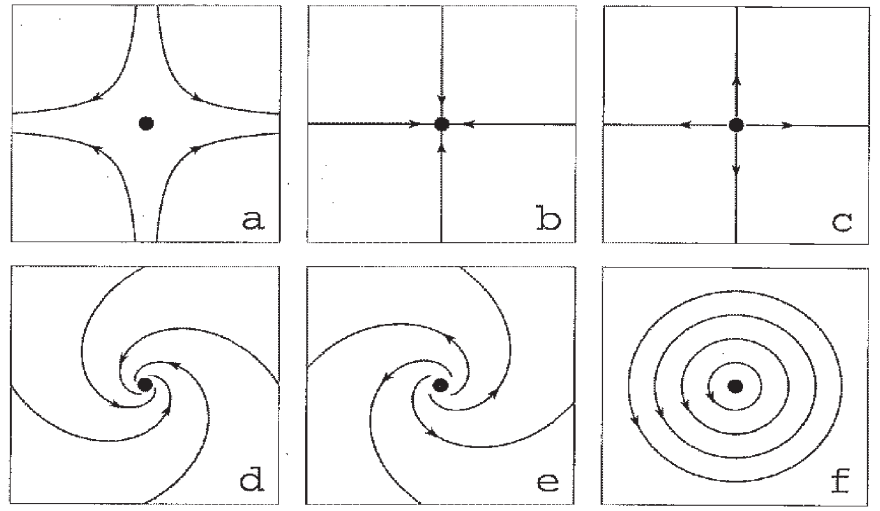
\includegraphics[width=.7\linewidth]{Pics/4.18.png}
\end{figure}

\begin{table}[H]
  \footnotesize
  \begin{tabular}{ll}
    a) saddle point    & e) unstable spiral\\
    b) stable node     & f) center/elliptic fixed point\\
    c) unstable node   & g) degenerate cases\\
    d) stable spiral   &
  \end{tabular}
\end{table}

A two-dimensional system can be characterized with the eigenvalues like so:
\begin{itemize}
  \item $\lambda_1 < 0, \lambda_2 < 0$: stable node
  \item $\lambda_1 > 0, \lambda_2 < 0$: saddle point
  \item $\lambda_1 > 0, \lambda_2 > 0$: usntable point
  \item $\lambda_1 = 0, \lambda_2 = 0$: non-isolated fixed point
  \item $\lambda_{1.2} \neq \mathbb{R}, \textup{Re}(\lambda_{1,2}) = 0$: center
  \item $\lambda_{1.2} \neq \mathbb{R}, \textup{Re}(\lambda_{1,2}) > 0$: unstable spiral
  \item $\lambda_{1.2} \neq \mathbb{R}, \textup{Re}(\lambda_{1,2}) < 0$: stable spiral
\end{itemize}

Alternativ characterization instead of with the eigenvalues $\lambda_1, \lambda_2$ with trace and determinant of A:
\begin{equation}
  \begin{split}
    \tau &= \textup{tr} = a_{11} + a_{22}\\
    \Delta &= \textup{det}(A) = a_{11}a_{22} - a_{12}a_{21}
  \end{split}
\end{equation}
Connection with the eigenvalues:
\begin{equation}
  \lambda_{1,2} = \frac{1}{2}\left(\tau \pm \sqrt{\tau^2 - 4\Delta}\right)
\end{equation}
and
\begin{equation}
  \Delta = \lambda_1 \lambda_2, \;\;\; \tau = \lambda_1 + \lambda_2
\end{equation}

In the following figure the classification of fixed points based on the properties of $\tau$ and $\Delta$ is shown graphically.
\begin{figure}[H]
  \centering
  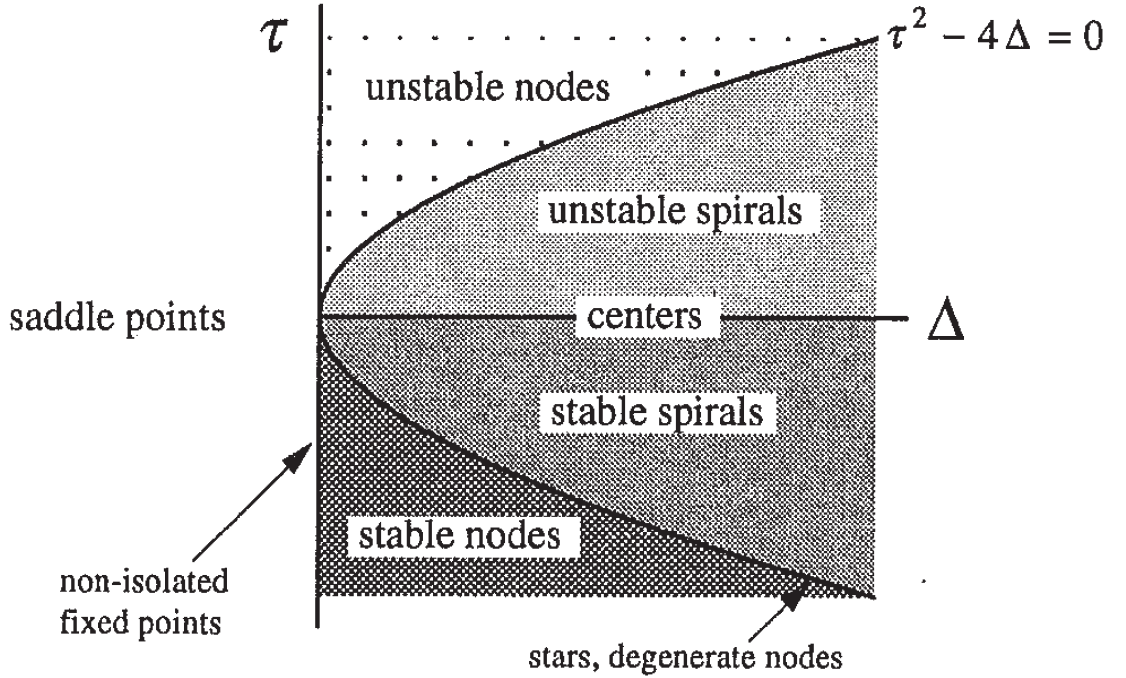
\includegraphics[width=.7\linewidth]{Pics/4.19.png}
\end{figure}

If one is only interested in the stability of $\textbf{x}^*$ (and not in a further classification into nodes,
spirals, etc.), the fixed point $\textbf{x}^* = 0$ of a dynamical system is
\begin{itemize}
  \item asymptotically stable, if
  \begin{equation}
    \textup{Re}(\lambda_i) < 0
  \end{equation}
  holds for all eigenvalues $\lambda_i$ of $A$

  \item stable, if
  \begin{equation}
    \textup{Re}(\lambda_i) \leq 0
  \end{equation}
  holds for all eigenvalues $\lambda_i$ of $A$

  \item usntable, if
  \begin{equation}
    \textup{Re}(\lambda_i) > 0
  \end{equation}
  holds for at least one eigenvalue $\lambda_i$ of $A$
\end{itemize}

\subsection{Nonlinear Systems}
\noindent\rule[\linienAbstand]{\linewidth}{\linienDicke}
In order to use the analysis of linear systems, we linearize the nonlinear system near the fixed point $x^*$. To this end, we consider small perturbations $u = x_1 - x^*_1, \; v = x_2 - x^*_2$ and deduce equations for $u$ and $v$ by expanding $f_1$ and $f_2$ into Taylor series. The temporal evolution of $(u, v)$ is thus given by
\begin{equation}
  \begin{pmatrix} \dot{u} \\ \dot{v} \end{pmatrix} =
  \begin{pmatrix} \frac{\partial f_1}{\partial x_1} & \frac{\partial f_1}{\partial x_2}\\
                  \frac{\partial f_2}{\partial x_1} & \frac{\partial f_2}{\partial x_1}
  \end{pmatrix}_{(x_1^*, x_2^*)} \cdot
  \begin{pmatrix} u \\ v \end{pmatrix} + \text{higher-order terms}
\end{equation}
The matrix
\begin{equation}
  A =   \begin{pmatrix} \frac{\partial f_1}{\partial x_1} & \frac{\partial f_1}{\partial x_2}\\
                        \frac{\partial f_2}{\partial x_1} & \frac{\partial f_2}{\partial x_1}
        \end{pmatrix}_{(x_1^*, x_2^*)}
\end{equation}
is the Jacobi matrix of the system near the fixed point $\textbf{x}^* = (x_1^*, x_2^*)$.\\

Example: Consider the system
\begin{equation}
  \begin{split}
    \dot{x} &= -x + x^3\\
    \dot{y} &= -2y
  \end{split}
\end{equation}
fixed points are:
\begin{equation}
  P_1 = (0, 0), \;\; P_2 = (1, 0), \;\; P_3 = (-1, 0).
\end{equation}
The Jacobi matrix of the system is
\begin{equation}
  A = \begin{pmatrix}
      -1+3x^2 & 0 \\
      0 & -2
  \end{pmatrix}
\end{equation}
The eigenvalues of $A$ are:
\begin{equation}
  P_1: \lambda_1 = -1, \lambda_2 = -2; \;\;\;\;\; P_2, P_3: \lambda_{1,2} = \pm 2
\end{equation}
Therefore $P_1$ is a stable node, and $P_2$ and $P_3$ are saddle points of the linearized system.\\

Intuitively: The linearization leads to the correct classification of the fixed points of nonlinear systems, if the fixed point type is described by an inequality and not an equality.\\

\textbf{Hartman-Grobman theorem}\\
If both eigenvalues $\lambda_1, \lambda_2$ of the corresponding system matrix $A$ fulfill the condition $\textup{Re}(\lambda_i) \neq 0$, then the behaviour of the nonlinear system is for sufficiently small perturbations topologically equivalent to the behaviour of the linearized system.\\

\textbf{Classification of fixed points into robust and marginal cases}\\
Robust: Nodes, spirals, saddle points\\
Marginal: centers/elliptic fixed points, degenerate cases

\subsection{Bifurications}
\noindent\rule[\linienAbstand]{\linewidth}{\linienDicke}
